\documentclass[border=2pt]{standalone}
\usepackage{times,amsmath,tikz}
\usetikzlibrary{arrows.meta,positioning}
\begin{document}
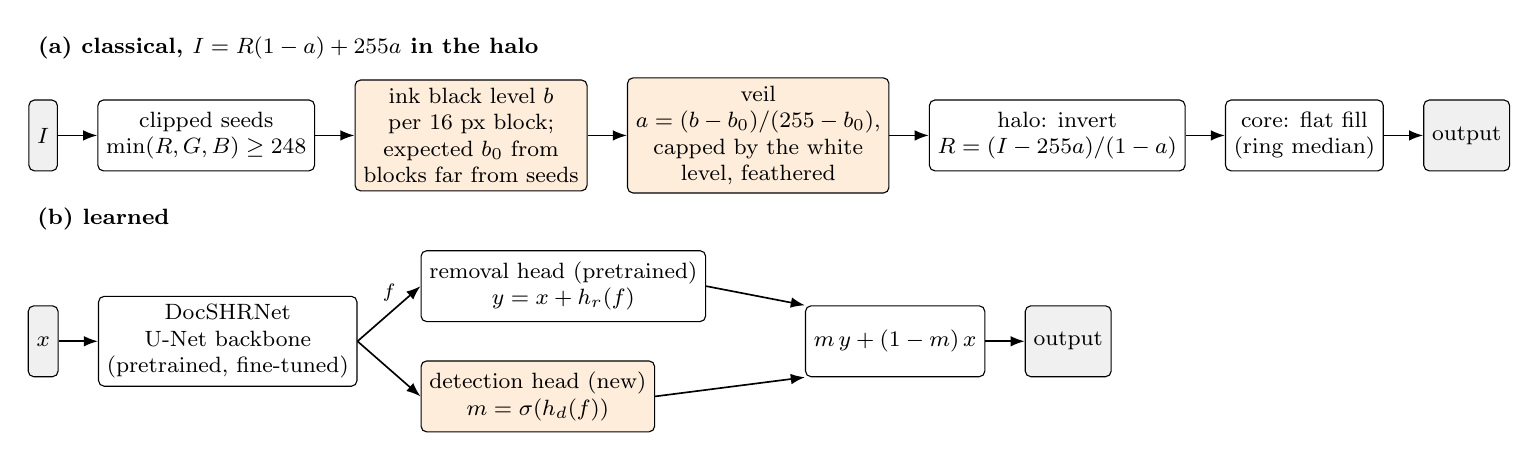
\begin{tikzpicture}[font=\footnotesize, node distance=5mm and 5mm,
  box/.style={draw,rounded corners=2pt,align=center,minimum height=9mm,inner sep=3pt,fill=white},
  data/.style={box,fill=black!6}, new/.style={box,fill=orange!14},
  arr/.style={-{Latex[length=1.8mm]},semithick}, lab/.style={font=\footnotesize\bfseries,anchor=west}]
% classical
\node[data] (x) {$I$};
\node[box,right=of x] (seed) {clipped seeds\\$\min(R,G,B)\ge 248$};
\node[new,right=of seed] (ink) {ink black level $b$\\per 16 px block;\\expected $b_0$ from\\blocks far from seeds};
\node[new,right=of ink] (veil) {veil\\$a=(b-b_0)/(255-b_0)$,\\capped by the white\\level, feathered};
\node[box,right=of veil] (inv) {halo: invert\\$R=(I-255a)/(1-a)$};
\node[box,right=of inv] (core) {core: flat fill\\(ring median)};
\node[data,right=of core] (y) {output};
\foreach \a/\b in {x/seed,seed/ink,ink/veil,veil/inv,inv/core,core/y} \draw[arr] (\a)--(\b);
\node[lab] at ([yshift=4mm]x.west |- ink.north) {(a) classical, $I=R(1-a)+255a$ in the halo};
% DL
\node[data,below=17mm of x] (x2) {$x$};
\node[box,right=of x2] (net) {DocSHRNet\\U-Net backbone\\(pretrained, fine-tuned)};
\node[box,right=8mm of net,yshift=7mm] (rem) {removal head (pretrained)\\$y=x+h_r(f)$};
\node[new,right=8mm of net,yshift=-7mm] (det) {detection head (new)\\$m=\sigma(h_d(f))$};
\node[box] (mix) at ([xshift=24mm]rem.east |- net) {$m\,y+(1-m)\,x$};
\node[data,right=of mix] (y2) {output};
\draw[arr] (x2)--(net); \draw[arr] (net.east)--(rem.west) node[midway,above,font=\scriptsize,yshift=1pt] {$f$}; \draw[arr] (net.east)--(det.west);
\draw[arr] (rem.east)--(mix.north west); \draw[arr] (det.east)--(mix.south west); \draw[arr] (mix)--(y2);
\node[lab] at ([yshift=4mm]x2.west |- rem.north) {(b) learned};
\end{tikzpicture}
\end{document}
